\documentclass[UTF8, 10pt, a4paper, oneside]{ctexart}
\usepackage{amsmath}
\usepackage{amsthm}
\usepackage{amsfonts}
\usepackage{amssymb}
\usepackage{amstext}
\usepackage[version=4]{mhchem}% 规范:chemfig中键线式放缩为0.5;结构简式放缩为0.6;高分子链节\polymerdelim[delimiters={[]},height=4pt, depth=4pt, indice=n]{left}
\usepackage{chemfig}
\setcharge{shortcuts=true}
\usepackage{geometry}
\usepackage{changepage}
\usepackage{paralist}
\usepackage{multicol}
\usepackage{graphicx}
\usepackage{polyglossia}
\usepackage{extarrows}
\setotherlanguages{russian}
\newfontfamily\russianfont{Times New Roman}
\geometry{left=1.27cm, right=1.27cm, top=1.27cm, bottom=1.5cm}
\linespread{1.5}
\title{\vspace{-2em}过教材\quad 选择性必修三\quad 有机化学基础\quad 参考答案\vspace{-2em}}
\author{}
\date{\textcolor{white}{\today}\vspace{-3em}}
\pagestyle{plain}

\newcommand{\blank}{ \underbar{\quad$\blacktriangle$\quad} }% 空格样式
\newcommand{\fs}[1]{{\fangsong #1}}% 使用仿宋
\newcommand{\circled}[1]{{\small{\textcircled{\tiny{#1}}}}}% 圈圈数字
\newcommand{\Romannumeral}[1]{\uppercase\expandafter{\romannumeral#1}}% 大写罗马数字
\newcommand{\chdots}{…\hspace{-0.15em}…}% 中文省略号调教

\theoremstyle{definition}
\newtheorem{exercise}{}
\newtheorem{subexercise}{}[exercise]% 用于兼容编号错误或是内含的高考题等

\theoremstyle{remark}
\newtheorem*{answer}{【答案】}
\newtheorem*{point}{【考点】}      % 考点&易错点
\newtheorem*{method}{【方法】}     %(可选)
\newtheorem*{explanation}{【解析】}     %

\theoremstyle{plain}
\newtheorem*{note}{【注】}  %(可选)

\begin{document}
\maketitle

\begin{exercise}
    1828年化学家维勒发现无机化合物\blank 通过加热可以直接转化为有机化合物尿素,尿素分子式为\blank ,结构式为\blank 。这促使了人们把生命力论对化合物分类改变为以\blank 为依据的分类方法。有机化合物中的原子以\blank 相结合,分子结构\blank,这决定了有机化合物种类,数量庞大。大多数有机物\blank 于水,\blank 燃烧。有机反应多为分子间的反应,一般反应速率\blank ,常伴有\blank ,产物比较复杂。官能团的\blank 和\blank、化学键的类型和\blank 是认识有机化合物结构和特征和有机反应的重要视角。
    \begin{answer}
        \begin{inparaenum}[\quad\textsuperscript{\arabic{enumi}}]
            \item[\setcounter{enumi}{1}\textsuperscript{\arabic{enumi}}] 氰酸铵
            \item $\ce{CH4ON2}$
            \item $\chemfig{[,0.6] C(=[:90]O)(-[:-30]NH_2)(-[:210]H_2N)}$
            \item 元素组成
            \item 共价键
            \item 复杂
            \item 不
            \item 可以
            \item 较小
            \item 副反应
            \item 种类
            \item 相互影响
            \item 极性
        \end{inparaenum}
    \end{answer}
\end{exercise}

\begin{exercise}
    按照碳骨架分类,有机物可以分为\blank 和\blank ,前者又可分为\blank 和\blank
    ,后者又可分为\blank (\blank 、\blank )和\blank (\blank 、\blank )。
    \blank 叫做官能团。
    常考的官能团结构及名称有:\blank 。
    丙烯酸中的官能团名称为\blank ,能发生的化学反应类型有\blank 。
    对羟基苯甲酸甲酯官能团名称为\blank ,能发生的化学反应类型有\blank 。
    3-溴-2-甲氧基-苯甲醛官能团名称为\blank ,能发生的化学反应类型有\blank 。
    丙烯酸分子中的化学键类型以及可能发生的反应类型\blank
    从化学键的极性角度分析乙醇和钠以及浓溴化氢溶液的反应:\blank
    从化学键和官能团角度分析甲烷与氯气,乙烯和溴的四氯化碳溶液的反应\blank。
    \begin{answer}
        \begin{inparaenum}[\quad\textsuperscript{\arabic{enumi}}]
            \item[\setcounter{enumi}{1}\textsuperscript{\arabic{enumi}}] 链状化合物
            \item 环状化合物
            \item 脂肪烃
            \item 脂肪烃衍生物
            \item 脂环化合物
            \item 脂环烃
            \item 脂环烃衍生物
            \item 芳香族化合物
            \item 芳香烃
            \item 芳香烃衍生物
            \item 决定有机化合物特性的原子或原子团
            \item \fs{略 [选必三P5 表1-1]}
            \item 碳碳双键、羧基
            \item 取代反应(酯化反应)、加成反应、还原反应、中和反应
            \item 羟基、酯基
            \item 中和反应、氧化反应、水解反应、氨解反应(生成酰胺)
            \item 碳溴键、醛基、醚键
            \item 氧化反应、还原反应、加成反应、取代反应、消去反应
            \item 共价键($\sigma$键、$\pi$键);加成反应、氧化反应、中和反应、取代反应(酯化反应)、还原反应
            \item $\ce{O-H}$键极性较大,使得氢带正电,易被钠的强还原性攻击;$\ce{C-OH}$键极性较大,易被亲核试剂$\ce{Br-}$取代
            \item 甲烷中没有典型官能团,其中的$\ce{C-H}$键均裂,引发自由基链式反应;乙烯中碳碳双键$\pi$电子云密度高,而与$\ce{Br2}$极化后生成的$\ce{Br+}$发生亲电加成
        \end{inparaenum}
    \end{answer}
\end{exercise}

\begin{exercise}
    \blank 叫同分异构现象,\blank 互为同分异构体。同分异构有构造异构和立体异构,构造异构有\blank ,立体异构有\blank 。戊烷的同分异构体结构式及命名\blank 。丁烯的同分异构体结构式及命名\blank 。二氯苯的同分异构体结构式及命名\blank。 $\ce{C2H6O}$的同分异构体结构式及命名\blank。 二氯甲烷是否存在对映异构,氯溴碘代甲烷呢,说明理由\blank 。
    \begin{answer}
        \begin{inparaenum}[\quad\textsuperscript{\arabic{enumi}}]
            \item[\setcounter{enumi}{1}\textsuperscript{\arabic{enumi}}] 化合物具有相同的分子式,但具有不同结构的现象
            \item 具有同分异构现象的化合物
            \item 碳架异构、位置异构、官能团异构
            \item 顺反异构、对映异构\vspace{0.5em}\\
            \item $\mathop{\chemfig{[,0.5]-[:30]-[:-30]-[:30]-[:-30]}}\limits_{\mbox{\kaishu 正戊烷}}$、$\mathop{\chemfig{[,0.5]-[:30](-[2])-[:-30]-[:30]}}\limits_{\mbox{\kaishu 异戊烷}}$、$\mathop{\chemfig{[,0.5]-[:30](-[2])(-[:-60])-[:-30]}}\limits_{\mbox{\kaishu 新戊烷}}$
            \item $\mathop{\chemfig{[,0.5]=^-[:30]-[:-30]}}\limits_{\mbox{\kaishu 1-丁烯}}$、$\mathop{\chemfig{[,0.5]-[:30]=^-[:30]}}\limits_{\mbox{\kaishu 2-丁烯}}$、$\mathop{\chemfig{[,0.5]=(-[:30])(-[:-30])}}\limits_{\mbox{\kaishu 2-甲基-1-丙烯}}$、$\mathop{\chemfig{[,0.5]*4(----)}}\limits_{\mbox{\kaishu 环丁烷}}$、$\mathop{\chemfig{[:-30,0.5]*3(--(-[:30])-)}}\limits_{\mbox{\kaishu 1-甲基环丙烷}}$\\
            \item $\mathop{\chemfig{[,0.5]*6(-=-(-Cl)=(-Cl)-=)}}\limits_{\mbox{\kaishu 邻二氯苯}}$、$\mathop{\chemfig{[,0.5]*6(-=-(-Cl)=-(-Cl)=)}}\limits_{\mbox{\kaishu 间二氯苯}}$、$\mathop{\chemfig{[,0.5]*6((-Cl)-=-(-Cl)=-=)}}\limits_{\mbox{\kaishu 对二氯苯}}$
            \item $\mathop{\ce{CH3CH2OH}}\limits_{\mbox{\kaishu 乙醇}}$、$\mathop{\ce{CH3OCH3}}\limits_{\mbox{\kaishu 二甲醚}}$\vspace{0.5em}\\
            \item 二氯甲烷不存在对映异构,因为其碳原子连接的取代基存在重复基团,该碳原子不构成手性中心;氯溴碘代甲烷存在对映异构,因为其碳原子连接的取代基不存在重复基团,该碳原子构成手性中心。
        \end{inparaenum}
    \end{answer}
    \begin{note}
        题\textsuperscript{7}对同分异构体书写的要求不明确,故按照“二氯苯含有苯环的同分异构体结构式及命名”给出答案。
    \end{note}
\end{exercise}
\newpage
\begin{exercise}
    \begin{multicols}{2}
        \noindent 完成11页第1题(有机物判断)\\
        完成11页第2题(有机物分子原子共面问题)\\
        完成11页第3题(有机物概念辨析)\\
        完成12页第4题(同分异构体判断)\\
        完成12页5题(官能团识别与名称)\\
        完成12页第6题(有机物官能团分类,读出其有机物名称)\\
        完成12页第7题(通过化学键和官能团分析有机化学反应)
    \end{multicols}

    \begin{answer}
        \fs{略}
    \end{answer}
\end{exercise}

\setcounter{exercise}{5}
\begin{subexercise}
    研究有机化合物的基本步骤:\blank 、\blank 、\blank 、\blank 。蒸馏是分离和提纯\blank 的常用方法,其原理是\blank 。蒸馏装置的仪器名称有\blank 。萃取包括液-液萃取和固-液萃取,前者是\blank 。使用的仪器有\blank ,仪器使用注意事项有\blank 。如何检查是否漏水:\blank 。萃取剂的选择\blank ,萃取的操作为\blank 、静置后分液的操作为\blank 。固液萃取是\blank 。
    \begin{answer}
        \begin{inparaenum}[\quad\textsuperscript{\arabic{enumi}}]
            \item[\setcounter{enumi}{1}\textsuperscript{\arabic{enumi}}] 分离、提纯
            \item 确定实验式
            \item 确定分子式
            \item 确定分子结构
            \item 液态互溶有机化合物
            \item 不同馏分沸点不同
            \item (含铁圈的)铁架台、酒精灯、陶土网、蒸馏烧瓶、温度计、直形冷凝管、牛角管、锥形瓶
            \item 利用待分离组分在两种不互溶的溶剂中的溶解度不同,将其从一种溶剂转移到另一种溶剂的过程
            \item (含铁圈的)铁架台、烧杯、(梨形)分液漏斗
            \item 装入液体总量不超过分液漏斗容积的 3/4、振荡时需倾斜漏斗(活塞端朝上),每隔几秒打开活塞排气(尤其易产气或低沸点溶剂),避免内部压力骤增导致液体喷溅、下层液体下口放,上层液体上口倒\chdots
            \item 可在漏斗中加入少量水后旋转活塞,观察是否渗漏
            \item 互不反应、互不相溶、萃取物溶解度大而杂质溶解度小(分配系数高)、易分离回收
            \item 检漏$\rightarrow$装液$\rightarrow$震荡\&排气$\rightarrow$静置分层$\rightarrow$分离
            \item 打开活塞缓慢放出下层液体至烧杯,接近排尽时关闭活塞,稍作静置后再放出残余液滴
            \item 用溶剂从固体物质中溶解出待分离组分的过程
        \end{inparaenum}
    \end{answer}
\end{subexercise}
\begin{subexercise}
    当晶体纯度不能达到要求时,应进行的操作为\blank 。重结晶是提纯\blank 有机化合物常用的方法,是利用\blank 。重结晶首先要选择适当的溶剂,要求杂质在此溶剂中溶解度\blank ,易于除去,被提纯的有机化合物在此溶剂中\blank ,能够进行\blank 。粗苯中含有少量的泥沙和氯化钠,提纯苯甲酸的步骤为:\blank (目的是\blank ) ,\blank (目的是\blank )、\blank (目的是\blank ) 、过滤(目的是\blank ),\blank (目的是\blank ),\blank (目的是\blank )。重结晶的收率计算公式为:\blank 。该实验中玻璃棒的作用为\blank 。如何检验提纯后的苯甲酸中氯化钠已被除尽\blank 。从氯化钠和硝酸钾的混合溶液中提取硝酸钾的操作为\blank 。从氯化钠和硝酸钾的混合溶液中提取氯化钠的操作为\blank 。硫酸铜溶液中得到无水硫酸铜晶体的操作为\blank 。
    \begin{answer}
        \begin{inparaenum}[\quad\textsuperscript{\arabic{enumi}}]
            \item[\setcounter{enumi}{1}\textsuperscript{\arabic{enumi}}] 重结晶
            \item 固体
            \item 用被提纯物质与杂质在同一溶剂中的溶解度不同而将杂质除去
            \item 很小或很大
            \item 受温度的影响较大
            \item 冷却结晶
            \item 加热溶解
            \item 使苯甲酸粗品充分溶解,提高产率
            \item 趁热过滤
            \item 除去泥沙,同时减少苯甲酸析出损耗
            \item 冷却结晶
            \item 使苯甲酸晶体析出,而可溶性杂质留在母液中
            \item 分离晶体与母液
            \item 冷水洗涤\vspace{0.5em}\\
            \item 除去晶体表面吸附的可溶性杂质
            \item 干燥称重
            \item 彻底去除溶剂,得到纯净的晶体
            \item $\dfrac{\text{纯化后产物质量}}{\text{粗产物质量}}\times 100\%$\vspace{0.5em}\\
            \item 搅拌、引流
            \item 取最后一次洗涤液,加入硝酸酸化的硝酸银,若无白色沉淀,则氯化钠已除尽
            \item 降温结晶
            \item 蒸发结晶
            \item 蒸发结晶
        \end{inparaenum}
    \end{answer}
\end{subexercise}
\begin{subexercise}
    \fs{[2024·广东卷]}提纯2.0 g苯甲酸粗品(含少量NaCl和泥沙)的过程如下。其中,操作X为\quad(\quad)
    \begin{figure}[ht!]
        \centering
        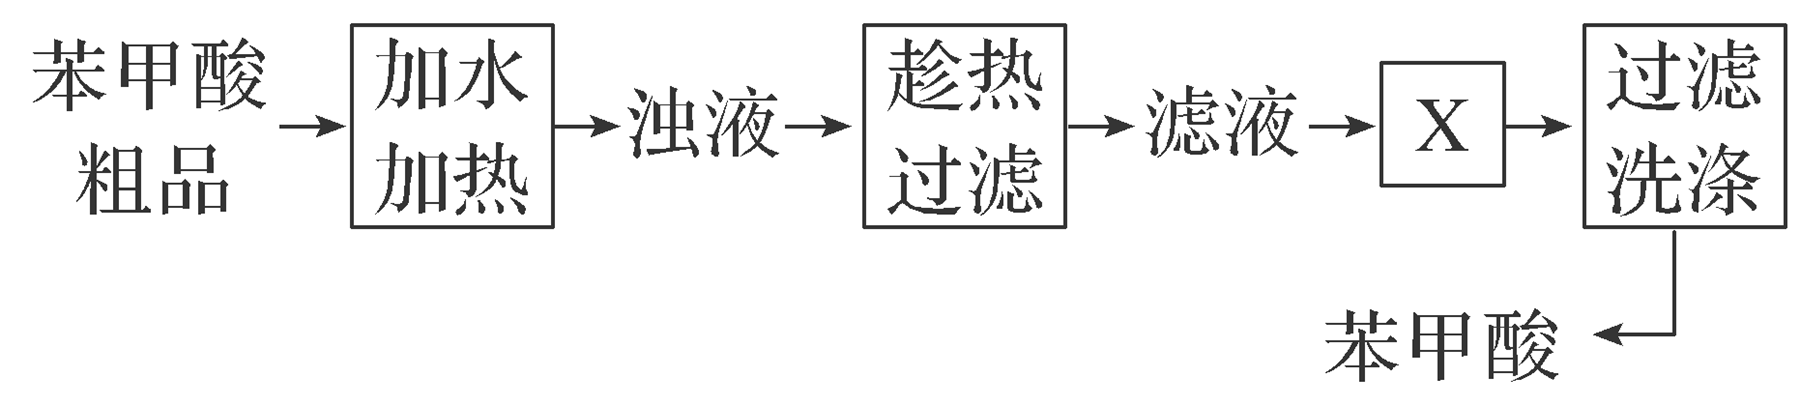
\includegraphics[width=0.5\textwidth, keepaspectratio]{assists/5.3.1.png}
    \end{figure}\vspace{-1.5em}
    \begin{center}
        \begin{inparaenum}[\qquad A. ]
            \item[\setcounter{enumi}{1}A. ] 加热蒸馏
            \item 加水稀释
            \item 冷却结晶
            \item 萃取分液
        \end{inparaenum}
    \end{center}
    \begin{answer}
        C
    \end{answer}
    \begin{point}
        教材实验、重结晶
    \end{point}
\end{subexercise}
\newpage
\begin{subexercise}
    \fs{[2023湖南3]}下列玻璃仪器在相应实验中选用不合理的是\quad(\quad)
    \begin{figure}[ht!]
        \centering
        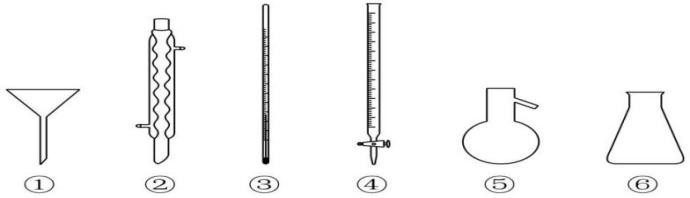
\includegraphics[width=0.4\textwidth, height=3cm]{assists/5.4.1.jpg}
    \end{figure}
    \begin{adjustwidth}{4em}{}
        \begin{asparaenum}[A. ]
            \item 重结晶法提纯苯甲酸:\circled{1}\circled{2}\circled{3}
            \item 蒸馏法分离$\ce{CH2Cl2}$和$\ce{CCl4}$:\circled{3}\circled{5}\circled{6}
            \item 浓硫酸催化乙醇制备乙烯:\circled{3}\circled{5}
            \item 酸碱滴定法测定NaOH溶液浓度:\circled{4}\circled{6}
        \end{asparaenum}
    \end{adjustwidth}
    \begin{answer}
        A
    \end{answer}
    \begin{point}
        实验器材的选取
    \end{point}
    \begin{explanation}
        重结晶法提纯苯甲酸时,不需要使用球形冷凝管,A选项不合理。
    \end{explanation}
\end{subexercise}
\begin{subexercise}
    \fs{[2023.6浙江]}苯甲酸是一种常用的食品防腐剂。某实验小组设计粗苯甲酸(含有少量NaCl和泥沙)的提纯方案如下,下列说法不正确的是\quad(\quad)
    \begin{figure}[ht!]
        \centering
        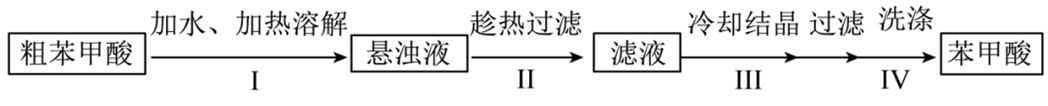
\includegraphics[width=0.8\textwidth, keepaspectratio]{assists/5.5.1.png}
    \end{figure}
    \begin{adjustwidth}{4em}{}
        \begin{asparaenum}[A. ]
            \item 操作\Romannumeral{1}中依据苯甲酸的溶解度估算加水量
            \item 操作\Romannumeral{2}趁热过滤的目的是除去泥沙和NaCl
            \item 操作\Romannumeral{3}缓慢冷却结晶可减少杂质被包裹
            \item 操作\Romannumeral{4}可用冷水洗涤晶体
        \end{asparaenum}
    \end{adjustwidth}
    \begin{answer}
        B
    \end{answer}
    \begin{point}
        教材实验、重结晶
    \end{point}
    \begin{explanation}
        趁热过滤的目的是除去泥沙,同时减少苯甲酸析出损耗,无法除去NaCl,B选项错误。
    \end{explanation}
\end{subexercise}
\begin{exercise}
    \begin{adjustwidth}{}{3cm}
        色谱法。当样品随着流动相经过固定相时,因样品中不同组分在两相间的分配不同而实现分离,这样的一类分离分析方法被称为色谱法。目前常用的固定相有硅胶、氧化铝等。1903年,俄国植物生理学家和化学家茨韦特(
        \begin{russian}
            M.C.Цвeт
        \end{russian},1872—1919)发表了第一篇关于色谱法的论文。他在玻璃管的一端塞上一团棉花,在管中填充碳酸钙粉末,再把溶有绿色植物色素的溶液自上而下注入玻璃管中。结果植物色素被碳酸钙粉末吸附,形成不同颜色的色带。他将吸附不同色素的碳酸钙分层取出,再用乙醇作溶剂,从植物色素中提取出叶绿素、叶黄素和胡萝卜素等较纯的组分。  此后,色谱法成为化学家分离、提纯有机化合物的重要方法之一。人们还开发了纸色谱、薄层色谱、气相色谱和高效液相色谱等多种色谱方法。
    \end{adjustwidth}\vspace{-14em}
    \begin{flushright}
        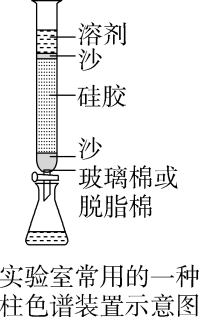
\includegraphics[width=2.5cm, keepaspectratio]{assists/chromatography.png}
    \end{flushright}\vspace{0.5em}

    \begin{subexercise}
        \fs{[2024·湖北卷]}萃取和柱色谱法可以从青蒿中提取分离青蒿素。\quad(\quad)
        \begin{answer}
            对。均可分离混合物的组分。
        \end{answer}
    \end{subexercise}
    \begin{subexercise}
        \fs{[2022·浙江卷]}用纸层析法分离铁离子和铜离子时,不能将滤纸条上的试样点浸入展开剂中。\quad(\quad)
        \begin{answer}
            对。纸层析法依靠不同物质在固定相(滤纸吸附的水分)和流动相(展开剂)中的分配系数差异实现分离。展开剂通过毛细作用沿滤纸上升,带动样品中各组分以不同速率迁移。若试样点直接接触展开剂,样品会溶解在溶剂中并扩散到溶液中,而非随展开剂上升。
        \end{answer}
    \end{subexercise}
\end{exercise}
\setcounter{subexercise}{0}
\addtocounter{exercise}{1}
\begin{subexercise}
    有机化合物的元素定量分析最早由德国化学家\blank 提出的,使用的仪器名称为\blank 。他用\blank 作氧化剂,将\blank 元素氧化为\blank ,用氢氧化钾浓溶液吸收\blank ,用无水氯化钙吸收\blank ,然后计算出有机化合物的\blank ,要确定其分子式,还需要测定\blank ,\blank 法是其中最精确快捷的方法,使用的仪器名称为\blank ,质谱图中最右侧质荷比为46,则说明相对分子质量为\blank ,可以确定其分子式为$\ce{C2H6O}$,则其可能的结构式为\blank 。经过\blank (仪器名称),得到\blank 图,从图中可以读出三组\blank 吸收峰,则可证明有机物为乙醇。氢原子具有磁性,若果用电磁波照射含氢元素的化合物,氢核\blank 而产生核磁共振现象,用\blank (仪器)可以记录有关信号,不同化学环境的氢原子共振时会吸收电磁波频率不同,谱图出现的位置不同,具有不同的\blank ,吸收峰的面积与\blank 成正比。化学位移一般用相对值表示,规定\blank 的氢原子信号的化学位移为零,多数有机化合物氢原子化学位移为\blank 范围。乙醇分子核磁共振氢谱有\blank 组,峰面积比为\blank 。X射线衍射图,可获得分子结构的有关数据,如\blank 等。青蒿素中的过氧基通过\blank 证明。
    \begin{answer}
        \begin{inparaenum}[\quad\textsuperscript{\arabic{enumi}}]
            \item[\setcounter{enumi}{1}\textsuperscript{\arabic{enumi}}] 李比希
            \item 李比希元素分析仪
            \item $\ce{CuO}$
            \item 碳
            \item $\ce{CO2}$
            \item $\ce{CO2}$
            \item $\ce{H2O}$
            \item 碳、氢、氧元素的质量分数,得到实验式
            \item 相对分子质量
            \item 质谱
            \item 质谱仪
            \item 46
            \item $\ce{CH3CH2OH}$、$\ce{CH3OCH3}$
            \item 红外光谱仪
            \item 红外光谱
            \item $\ce{C-H}$、$\ce{C-O}$、$\ce{O-H}$
            \item 会吸收特定频率电磁波的能量
            \item 核磁共振仪
            \item 化学位移
            \item 氢原子数
            \item $\ce{(CH3)4Si}$
            \item 0$\sim$10
            \item 3
            \item $3:2:1$
            \item 键长、键角等分子结构信息
            \item 化学反应
        \end{inparaenum}
    \end{answer}
\end{subexercise}
\begin{subexercise}
    \fs{[2023全国乙26]}元素分析是有机化合物的表征手段之一。按下图实验装置(部分装置略)对有机化合物进行C、H元素分析。回答下列问题:
    \begin{figure}[ht!]
        \centering
        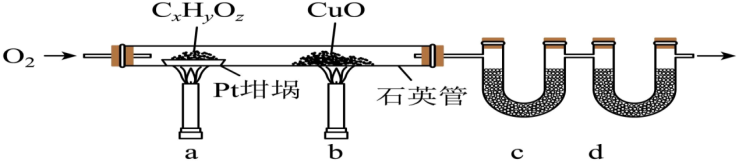
\includegraphics[width=0.5\textwidth, keepaspectratio]{assists/7.2.1.png}
    \end{figure}
    \begin{asparaenum}[(1)]
        \item 将装有样品的Pt坩埚和CuO放入石英管中,先\blank ,而后将已称重的U型管c、d与石英管连接,检查\blank 。依次点燃煤气灯\blank ,进行实验。
        \item $\ce{O2}$的作用有\blank 。CuO的作用是\blank (举1例,用化学方程式表示)。
        \item c和d中的试剂分别是\blank 、\blank (填标号)。c和d中的试剂不可调换,理由是\blank 。
        \begin{center}
            \begin{inparaenum}[\qquad A. ]
                \item[A. ] $\ce{CaCl2}$
                \item[\qquad B. ] NaCl
                \item[\qquad C. ] 碱石灰(CaO+NaOH)
                \item[\qquad D. ] $\ce{Na2SO3}$
            \end{inparaenum}
        \end{center}
        \item Pt坩埚中样品$\ce{C_xH_yO_z}$反应完全后,应进行操作:\blank 。取下c和d管称重。
        \item 若样品$\ce{C_xH_yO_z}$为0.0236g,实验结束后,c管增重0.0108g,d管增重0.0352g。质谱测得该有机物的相对分子量为118,其分子式为\blank 。
    \end{asparaenum}
    \begin{answer}
        \begin{inparaenum}[\quad\textsuperscript{\arabic{enumi}}]
            \item[\setcounter{enumi}{1}\textsuperscript{\arabic{enumi}}] 通入一定量的氧气
            \item 装置气密性
            \item b、a
            \item 氧化有机物、提供气流保证反应产物完全进入到c、d中
            \item $\ce{CO + CuO \xlongequal{\triangle} CO2 + Cu}$
            \item A
            \item C
            \item 碱石灰会吸收$\ce{H2O}$,干扰其测定
            \item 撤去煤气灯a、b,继续通入氧气,使反应产物完全进入到c、d中,冷却装置
            \item $\ce{C4H6O4}$
        \end{inparaenum}
    \end{answer}
    \begin{point}
        定量实验、热重分析
    \end{point}
    \begin{explanation}
        题\textsuperscript{10}:可知$n(C):n(H):n(O)=\dfrac{0.0352}{12+32}:\dfrac{0.0108}{18}\times 2 :\dfrac{0.0236-n(C)\times 12-n(H)\times 1}{16}=2:3:2$,又$M(\ce{C_xH_yO_z})=118$,解得其分子式为$\ce{C4H6O4}$。
    \end{explanation}
\end{subexercise}
\setcounter{subexercise}{0}
\addtocounter{exercise}{1}
\begin{subexercise}
    \begin{multicols}{2}
        \noindent 完成21页第1题(分离方式的选择)\\
        完成21页第2题(有机物分子分析)\\
        完成21页第3题(质谱图信息获取与分析)
    \end{multicols}
    \begin{answer}
        \fs{略}
    \end{answer}
    \newpage
\end{subexercise}
\begin{subexercise}
    \fs{[2024·湖北卷]}关于物质的分离、提纯,下列说法错误的是\quad(\quad)
    \begin{adjustwidth}{4em}{}
        \begin{asparaenum}[A. ]
            \item 蒸馏法分离$\ce{CH2Cl2}$和$\ce{CCl4}$
            \item 过滤法分离苯酚和$\ce{NaHCO3}$溶液
            \item 萃取和柱色谱法从青蒿中提取分离青蒿素
            \item 重结晶法提纯含有少量食盐和泥沙的苯甲酸
        \end{asparaenum}
    \end{adjustwidth}
    \begin{answer}
        B
    \end{answer}
    \begin{point}
        物质的分离提纯
    \end{point}
    \begin{explanation}
        $\ce{CH2Cl2}$沸点为$39.8^\circ$C,$\ce{CCl4}$沸点为$76.5^\circ$C,沸点差异较大,可以通过蒸馏分离,A选项正确;苯酚和$\ce{NaHCO3}$溶液应用萃取分液法分离,B选项错误;青蒿素不溶于水,可通过有机溶剂乙醚低温萃取或柱色谱法分离得到青蒿素,C选项正确;苯甲酸在水中的溶解度受温度影响变化较大且苯甲酸与食盐在水中溶解度相差较大,故可以用重结晶法提纯,D选项正确。
    \end{explanation}
\end{subexercise}
\begin{subexercise}
    \fs{[2024·湖北卷]}鹰爪甲素(如图)可从治疗疟疾的有效药物鹰爪根中分离得到。下列说法错误的是\quad(\quad)
    \begin{adjustwidth}{4em}{}
        \begin{asparaenum}[A. ]
            \item 有5个手性碳
            \item 在120$^\circ$C条件下干燥样品
            \item 同分异构体的结构中不可能含有苯环
            \item 红外光谱中出现了3000 cm$^{-1}$以上的吸收峰
        \end{asparaenum}
    \end{adjustwidth}\vspace{-8em}
    \begin{flushright}
        $\chemfig{[,0.5]*6(-(-[:210](-[6])-[:150]-[2]?)-O-O-(-[:150])(-[:30]=^[:-30]-[:30](-[2]OH)-[:-30](-[6]OH)(-[:30])(-[:-30]))-?-)}$
    \end{flushright}\vspace{-0.5em}
    \begin{answer}
        B
    \end{answer}
    \begin{point}
        物质的分离提纯
    \end{point}
    \begin{explanation}
        \begin{adjustwidth}{}{14em}
            如右图所示,鹰爪甲素有5个手性碳,A选项正确;鹰爪甲素中含有过氧键($\ce{-O-O-}$)温度过高时易断裂(类比青蒿素只能低温萃取),故不能在120$^\circ$C条件下干燥样品,B选项错误;由结构简式可知,鹰爪甲素不饱和度$\Omega = 3$,而苯环的不饱和度$\Omega = 4$,故同分异构体的结构中不可能含有苯环,C选项正确;$\ce{O-H}$的吸收峰在未形成氢键时,通常在 3600–3700cm$^{-1}$附近,表现为尖锐的峰,结合氢键后吸收峰向低频移动,范围扩大至 3200–3600cm$^{-1}$,峰形变宽,故D选项正确。
        \end{adjustwidth}\vspace{-12em}
        \begin{flushright}
            $\chemfig{[,0.5]*6(-\charge{[circle]300:1mm=*}{}(-[:210]\charge{[circle]220:1.5mm=*}{}(-[6])-[:150]-[2]?)-O-O-\charge{[circle]90:0.5mm=*}{}(-[:150])(-[:30]=^[:-30]-[:30]\charge{[circle]270:1.5mm=*}{}(-[2]OH)-[:-30](-[6]OH)(-[:30])(-[:-30]))-\charge{[circle]135:0.5mm=*}{}?-)}$
        \end{flushright}\vspace{4em}
    \end{explanation}
\end{subexercise}
\begin{exercise}
    \begin{multicols}{2}
        \noindent 完成21页第4题(核磁共振氢谱)\\
        完成22页5题(重结晶除杂)\\
        完成22页第6题(李比希元素分析与质谱分析)\\
        完成22页第7题(实验室与分子式确定)\\
        完成22页第8题(核磁共振氢谱与有机物命名)\\
        完成22页第9题(有机物分子推断综合利用)\\
        完25页第1题(分离方式的选择)\\
        完成25页第2题(有机物分子分析)\\
        完成25页第3题(质谱图信息获取与分析)\\
        完成25页第4题(核磁共振氢谱)\\
        完成26页5题(重结晶除杂)\\
        完成26页第6题(李比希元素分析与质谱分析)\\
        完成26页第7题(实验室与分子式确定)\\
        完成26页第8题(核磁共振氢谱与有机物命名)
    \end{multicols}
    \begin{answer}
        \fs{略}
    \end{answer}
\end{exercise}
\begin{exercise}
    仅含碳和氢两种元素的有机物称为\blank ,其碳原子的\blank 和\blank ,是预测化学反应中烃分子可能断键部位与相应反应类型的主要依据。凡士林和石蜡的主要成分为\blank 。烷烃中碳原子的杂化方式为\blank ,化学键类型为\blank ,甲烷的溶解性\blank ,常温下能否与酸性高锰酸钾、强酸强碱和溴的四氯化碳溶液反应\blank ,说明甲烷的化学性质\blank 。写出辛烷(汽油成分之一)燃烧的反应:\blank 。从化学键与官能团角度分析乙烷与氯气生成一氯乙烷的反应及反应类型\blank 。乙烷与氯气光照下产物为(写键线式和命名)\blank 。\blank 互称同系物,甲烷的同系物熔沸点变化规律\blank 。
    \begin{answer}
        \begin{inparaenum}[\quad\textsuperscript{\arabic{enumi}}]
            \item[\setcounter{enumi}{1}\textsuperscript{\arabic{enumi}}] 碳氢化合物(烃)
            \item 饱和程度
            \item 化学键的类型
            \item 烷烃
            \item $sp^3$
            \item $\sigma$键
            \item 难溶于水
            \item 不能
            \item 比较稳定
            \item $\ce{2C8H18 + 25O2 \xlongequal{\text{点燃}} 16CO2 + 18H2O}$
            \item 乙烷中没有典型官能团,其中的$\ce{C-H}$键均裂,引发自由基链式反应
            \item $\mathop{\chemfig{[,0.5](-[:150]Cl)-}}\limits_{\mbox{\kaishu 1-氯乙烷}}$、
            $\mathop{\chemfig{[,0.5](-[:210]Cl)(-[:150]Cl)-}}\limits_{\mbox{\kaishu 1,1-二氯乙烷}}$、
            $\mathop{\chemfig{[,0.5](-[:150]Cl)--[:-30]Cl}}\limits_{\mbox{\kaishu 1,2-二氯乙烷}}$、
            $\mathop{\chemfig{[,0.5](-[:260]Cl)(-[:210]Cl)(-[:150]Cl)-}}\limits_{\mbox{\kaishu 1,1,1-三氯乙烷}}$、
            $\mathop{\chemfig{[,0.5](-[:210]Cl)(-[:150]Cl)--[:-30]Cl}}\limits_{\mbox{\kaishu 1,1,2-三氯乙烷}}$、
            $\mathop{\chemfig{[,0.5](-[:210]Cl)(-[:150]Cl)-(-[:30]Cl)(-[:-30]Cl)}}\limits_{\mbox{\kaishu 1,1,2,2-四氯乙烷}}$、
            $\mathop{\chemfig{[,0.5](-[:260]Cl)(-[:210]Cl)(-[:150]Cl)--[:-30]Cl}}\limits_{\mbox{\kaishu 1,1,1,2-四氯乙烷}}$、\\
            $\mathop{\chemfig{[,0.5](-[:260]Cl)(-[:210]Cl)(-[:150]Cl)-(-[:-30]Cl)(-[:30]Cl)}}\limits_{\mbox{\kaishu 1,1,1,2,2-五氯乙烷}}$、
            $\mathop{\chemfig{[,0.5](-[:260]Cl)(-[:210]Cl)(-[:150]Cl)-(-[:-30]Cl)(-[:30]Cl)(-[:280]Cl)}}\limits_{\mbox{\kaishu 六氯乙烷}}$\vspace{0.5em}\\
            \item 结构相似、分子组成上相差一个或若干个$\ce{CH2}$原子团的化合物
            \item 碳数越大,沸点越高;支链越多,沸点越低
        \end{inparaenum}
    \end{answer}
    \begin{note}
        题\textsuperscript{12}还应有无机产物$\ce{HCl}$。但由于$\ce{HCl}$没有键线式,故按照“乙烷与氯气光照下的有机产物”给出答案。
    \end{note}
\end{exercise}
\begin{exercise}
    \begin{multicols}{2}
        \noindent 完成32页第1题(烷烃的取代反应)\\
        完成32页第2题(烷烃的性质)\\
        完成33页第3题(同分异构判断)\\
        完成33页第4题(同系物判断)\\
        完成33页5题(同分异构体判断)\\
        完成33页第6题(同分异构体判断)\\
        完成33页第7题(同分异构体判)\\
        完成33页第8题(伯仲叔季碳)\\
    \end{multicols}
    \begin{answer}
        \fs{略}
    \end{answer}
\end{exercise}
\setcounter{subexercise}{0}
\addtocounter{exercise}{1}
\begin{subexercise}
    乙烯的结构式为\blank ,乙烯中碳原子的杂化方式为\blank ,化学键类型为\blank ,乙烯可以发生的反应类型有\blank 。丙烯与溴水、氯化氢和水反应的化学方程式为\blank 氯乙烯、异丁烯加聚反应方程式为\blank 2-丁烯的两种结构为\blank ,稳定的是\blank 原因是\blank 1,3-丁二烯发生1,2和1,4加成的反应方程式\blank 1,3-丁二烯发生加聚反应的化学方程式为\blank 乙炔的结构式为\blank ,乙炔中碳原子的杂化方式为\blank ,化学键类型为\blank ,乙炔可以发生的反应类型有\blank 乙炔的制备原理为\blank ,饱和食盐水代替水的目的是\blank 如何除杂\blank ,怎样检验乙炔\blank 乙炔属于可燃性气体,点燃前要\blank ,防止\blank 。乙炔与酸性高锰酸钾或溴的四氯化碳反应实验现象为\blank ,点燃乙炔实验现象为\blank 。乙炔与中缓慢加入溴水分别的反应为\blank 产物名称分别为\blank 。乙炔分别与等物质的量的氯化氢和水反应产物名称分别为\blank 。乙炔可以制备高分子导电材料,化学方程式为\blank 。
    \begin{answer}
        \begin{inparaenum}[\quad\textsuperscript{\arabic{enumi}}]
            \item[\setcounter{enumi}{1}\textsuperscript{\arabic{enumi}}] $\chemfig{[,0.6]C(-[:120]H)(-[:-120]H)=C(-[:60]H)(-[:-60]H)}$\vspace{0.5em}
            \item $sp^2$
            \item 共价键($\pi$键、$\sigma$键)
            \item 加成反应、氧化反应、取代反应\\
            \item $\ce{CH3CH=CH2 + Br2 -> CH3CHBr-CH2Br}$;\\$\ce{CH3CH=CH2 + HCl ->T[催化剂] CH3CHCl-CH3}$(主要)、$\ce{CH3CH=CH2 + HCl ->T[催化剂] CH3CH2-CH2Cl}$(次要);\\$\ce{CH3CH=CH2 + H2O ->T[催化剂][T,P] CH3CH(OH)-CH3}$(主要)、$\ce{CH3CH=CH2 + H2O ->T[催化剂][T,P] CH3CH2-CH2OH}$(次要)\\
                \item $\ce{n CH2=CHCl ->T[催化剂]}\chemfig{[,0.6]-[@{left,0.5},0.5]CH_2-CHCl-[@{right,0.5},0.5]}\polymerdelim[delimiters={[]},height=4pt, depth=4pt, indice=n]{left}{right}$\hspace{0.5em};$\ce{n CH2=C(CH2)2 ->T[催化剂]}\chemfig{[,0.6]-[@{left,0.5}]C(-[2]CH_3)(-[6]CH_3)-CH_2-[@{right,0.5}]}\polymerdelim[delimiters={[]},height=4pt, depth=4pt, indice=n]{left}{right}$
                \item $\chemfig{[,0.4](-[:150])=^-[:30]}$、$\chemfig{[,0.4](-[:150])=^-[:-30]}$\\
                \item 反式结构$\chemfig{[,0.4](-[:150])=^-[:-30]}$
                \item 顺式结构中,双键两侧的两个甲基位于同一侧,彼此靠近,导致较大的空间排斥,更不稳定\\
                \item $\ce{CH2=CH-CH=CH2 + X2 ->}\chemfig{[,0.6]CH_2(-[6]X)-CH(-[6]X)-CH=CH_2}$;$\ce{CH2=CH-CH=CH2 + X2 ->}\chemfig{[,0.6]CH_2(-[6]X)-CH=CH-CH_2(-[6]X)}$\\
                \item $\ce{n CH2=CH-CH=CH2 ->T[催化剂]}\chemfig{[,0.6]-[@{left,0.5}]CH_2-CH=CH-CH_2-[@{right,0.5}]}\polymerdelim[delimiters={[]},height=4pt, depth=4pt, indice=n]{left}{right}$
                \item $\ce{H-C#C-H}$
                \item $sp$
                \item 共价键($\pi$键、$\sigma$键)
                \item 加成反应、氧化反应、取代反应
                \item $\ce{CaC2 + 2H2O -> Ca(OH)2 + HC#CH}$
                \item 减缓反应速率
                \item 先后通过饱和$\ce{CuSO4}$溶液、浓硫酸
                \item 燃烧、通过高锰酸钾溶液、通过溴的四氯化碳溶液、\textbf{与硝酸银氨溶液反应生成灰白色沉淀}\chdots
                \item 验纯
                \item 混合气体被点燃时因反应速度过快、能量瞬间释放而导致爆炸
                \item 溶液褪色
                \item 产生明亮火焰并伴有浓烟
                \item $\ce{HC#CH + Br2 -> CHBr=CHBr}$、$\ce{CHBr=CHBr + Br2 -> CHBr2-CHBr2}$
                \item 1,2-二溴乙烯、1,1,2,2-四溴乙烷
                \item 氯乙烯;乙醛
                \item $\ce{n HC#CH ->T[催化剂]}\chemfig{[,0.6]-[@{left,0.5},0.5]CH=CH-[@{right,0.5},0.5]}\polymerdelim[delimiters={[]},height=4pt, depth=4pt, indice=n]{left}{right}$
        \end{inparaenum}
    \end{answer}
    \begin{note}
        默认所有加成反应催化剂不为过氧化物。题\textsuperscript{10}未明确反应物,按照卤素($\ce{X2}$)给出答案。乙炔与硝酸银氨溶液反应是其特征反应:$\ce{HC#CH + 2Ag(NH3)2^+ ->}\mathop{\ce{Ag2C2}}\limits_{\text{灰白色}}\ce{v + 2NH4^+ + 2NH3}$
    \end{note}
\end{subexercise}
\begin{subexercise}
    \fs{[2024·河北卷]}化合物X是由细菌与真菌共培养得到的一种天然产物,结构简式如图。下列相关表述错误的是\vspace{-0.5em}
    \begin{flushright}
        \quad(\quad)
    \end{flushright}\vspace{-3em}
    \begin{adjustwidth}{4em}{}
        \begin{asparaenum}[A. ]
            \item 可与$\ce{Br2}$发生加成反应和取代反应
            \item 可与$\ce{FeCl3}$溶液发生显色反应
            \item 含有4种含氧官能团
            \item 存在顺反异构
        \end{asparaenum}
    \end{adjustwidth}\vspace{-6.5em}
    \begin{adjustwidth}{}{6em}
        \begin{flushright}
            $\chemfig{[,0.5]*6((-HO)-=(-OH)-(-CHO)=(-[,0.7](=[:150,0.8]O)-[:30,0.8]*6(-(-OH)=(-Cl)-(-)=(-Cl)-(-O-[2])=))-(-[:150]-[:-150]=^[:150](-[2])(-[:-150]))=)}$
        \end{flushright}
    \end{adjustwidth}\vspace{-4em}
    \begin{answer}
        D
    \end{answer}
    \begin{point}
        顺反异构、官能团识别、酚羟基的性质、溴的加成
    \end{point}
    \begin{explanation}
        X中存在碳碳双键和烃基,分别可与溴加成或取代,A选项正确;X中存在酚羟基,可与$\ce{FeCl3}$溶液发生显色反应,B选项正确;X中含有羟基、羰基、醛基、醚键4种含氧官能团,C选项正确;顺反异构要求碳碳双键两侧所连的基团每端至少有一个与众不同,X不满足要求,D选项错误。
    \end{explanation}
\end{subexercise}
\begin{subexercise}
    \fs{[2024·甘肃卷]}下列实验操作对应的装置不正确的是\quad(\quad)
    \begin{figure}[h]
        \centering
        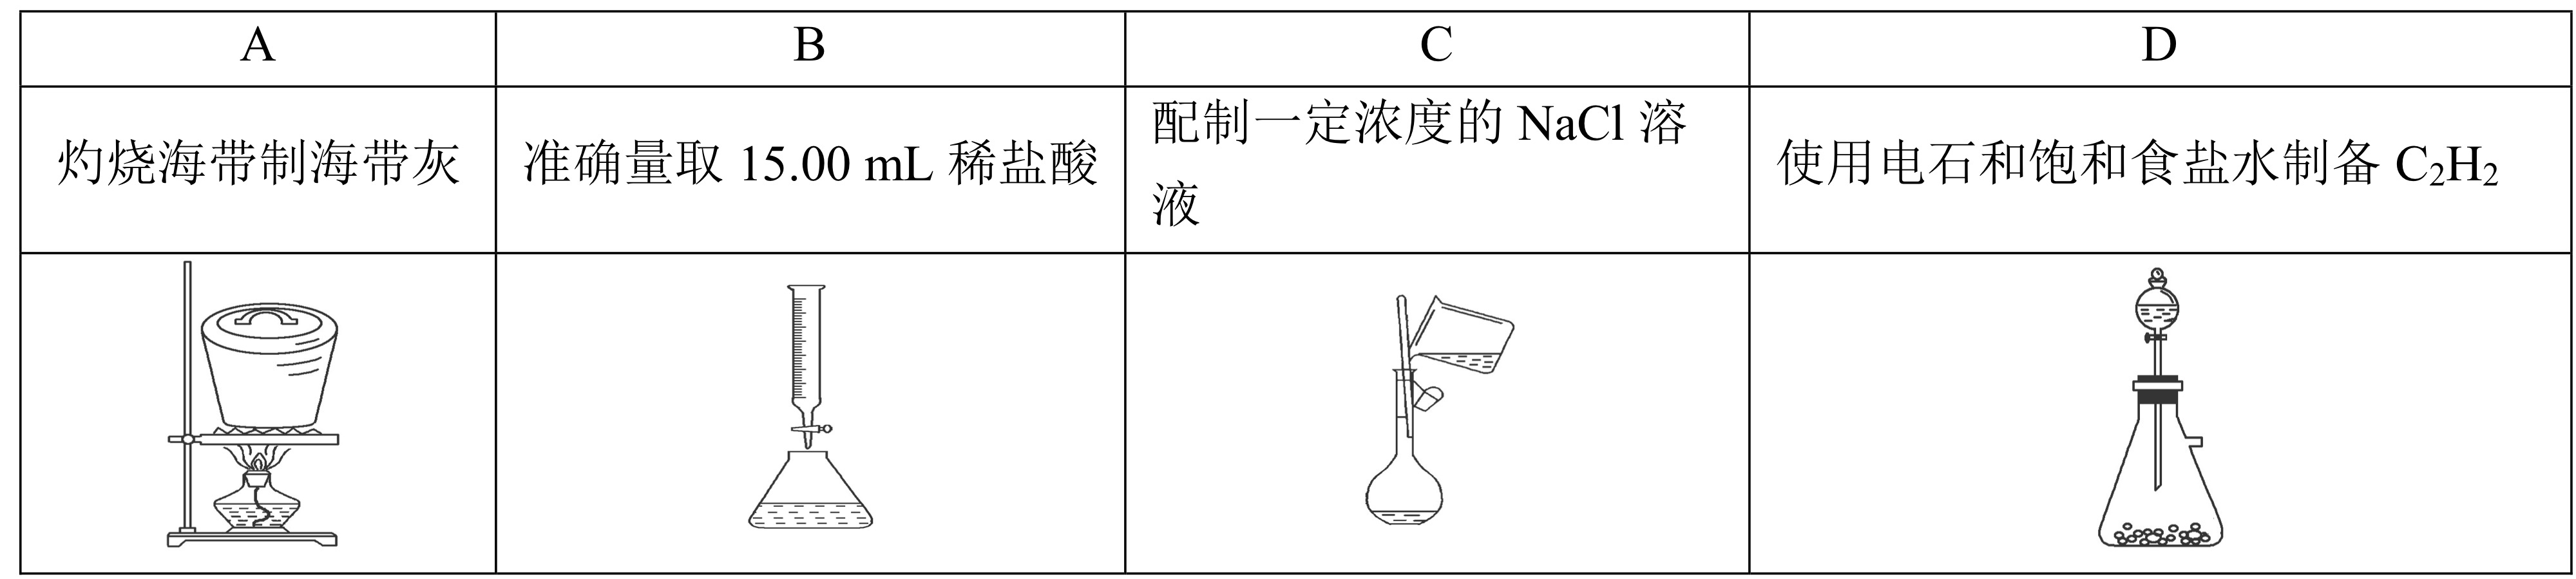
\includegraphics[width=0.8\textwidth, keepaspectratio]{assists/12.3.1.jpg}
    \end{figure}
    \begin{answer}
        A
    \end{answer}
    \begin{point}
        实验器材的选取
    \end{point}
    \begin{explanation}
        灼烧海带制海带灰需要在坩埚、泥三角、三脚架中进行,不需要使用陶土网,故A选项错误。
    \end{explanation}
\end{subexercise}
\begin{subexercise}
    聚乙炔可导电的原因是\blank ;乙炔在氧气中燃烧时放出大量的热,温度高达3000℃,因此常用它来\blank 。戊炔属于炔烃的同分异构体结构式及名称为\blank ;戊炔属于二烯烃的同分异构体结构式及名称为\blank ;戊炔属于环烯烃的同分异构体结构式及名称为\blank ;加氢可以得到2-甲基戊烷的炔烃可能的结构式及名称为\blank 。
    \begin{answer}
        \begin{inparaenum}[\quad\textsuperscript{\arabic{enumi}}]
            \item[\setcounter{enumi}{1}\textsuperscript{\arabic{enumi}}] 形成类似大$\pi$键的共轭双键,为电子沿链的移动提供了可能
            \item 焊接或切割金属\vspace{0.5em}\\
            \item $\mathop{\chemfig{[,0.5]~--[:30]-[:-30]}}\limits_{\mbox{\kaishu 1-戊炔}}$、$\mathop{\chemfig{[,0.5]-~--[:30]}}\limits_{\mbox{\kaishu 2-戊炔}}$、$\mathop{\chemfig{[,0.5]~-(-[:30])(-[:-30])}}\limits_{\mbox{\kaishu 3-甲基-1-丁炔}}$
            \item $\mathop{\chemfig{[,0.5]=^-[:30]=^-[:-30]}}\limits_{\mbox{\kaishu 1,3-戊二烯}}$、$\mathop{\chemfig{[,0.5]=^-[:30]-[:-30]=^}}\limits_{\mbox{\kaishu 1,4-戊二烯}}$、$\mathop{\chemfig{[,0.5]=^-[:30](=[2])-[:-30]}}\limits_{\mbox{\kaishu 2-甲基-1,3-丁二烯}}$\\
            \item $\mathop{\chemfig{[:18,0.5]*5(=----)}}\limits_{\mbox{\kaishu 环戊烯}}$、$\mathop{\chemfig{[,0.5]*4(--(-)=-)}}\limits_{\mbox{\kaishu 1-甲基环丁烯}}$、$\mathop{\chemfig{[,0.5]*4(=-(-)--)}}\limits_{\mbox{\kaishu 3-甲基环丁烯}}$、$\mathop{\chemfig{[,0.5]*4(--(=)--)}}\limits_{\mbox{\kaishu 甲亚基环丁烷}}$、$\mathop{\chemfig{[:-30,0.5]*3(--(-[:30]=^[:0])-)}}\limits_{\mbox{\kaishu 乙烯基环丙烷}}$、$\mathop{\chemfig{[,0.5]*3(-(=^-[:30])--)}}\limits_{\mbox{\kaishu 乙亚基环丙烷}}$、$\mathop{\chemfig{[:-30,0.5]*3(=-(-[:30]-[:-30])-)}}\limits_{\mbox{\kaishu 3-乙基环丙烯}}$、$\mathop{\chemfig{[:-30,0.5]*3(=-(-[:30])(-[:150])-)}}\limits_{\mbox{\kaishu 3,3-二甲基环丙烯}}$\\
            \item $\mathop{\chemfig{[,0.5]-[:30](=[2])-[:-30]-[:30]-[:-30]}}\limits_{\mbox{\kaishu 2-甲基戊烯}}$、$\mathop{\chemfig{[,0.5]-[:30](-[2])=^[:-30]-[:30]-[:-30]}}\limits_{\mbox{\kaishu 2-甲基-2-戊烯}}$、$\mathop{\chemfig{[,0.5]-[:30](-[2])-[:-30]=^[:30]-[:-30]}}\limits_{\mbox{\kaishu 4-甲基-2-戊烯}}$、$\mathop{\chemfig{[,0.5]-[:30](-[2])-[:-30]-[:30]=^[:-30]}}\limits_{\mbox{\kaishu 4-甲基戊烯}}$
        \end{inparaenum}
    \end{answer}
\end{subexercise}
\setcounter{subexercise}{0}
\addtocounter{exercise}{1}
\begin{subexercise}
    \begin{multicols}{2}
        \noindent 完42页第1题(同分异构体判断)\\
        完成42页第2题(乙烯乙炔就结构与性质)\\
        完成42页第3题(加成反应)\\
        完成42页第4题(原子共面问题)\\
        完成42页5题(丙烯的结构与性质)\\
        完成42页第6题(烯烃被高锰酸钾氧化)\\
        完成42页第7题(有机物研究)
    \end{multicols}
    \begin{answer}
        \fs{略}
    \end{answer}
\end{subexercise}
\begin{subexercise}

    \blank 叫做芳香烃,最简单的芳香烃为\blank 。苯是一种无色,有\blank 气味的液体,\blank 毒,\blank 于水,\blank 挥发,苯是一种重要的化工原料和\blank 。苯分别加入高锰酸钾和溴水中,振荡,实验现象为\blank ,实验结论为\blank 。苯分子的化学式为\blank ,结构式为\blank ,碳原子杂化方式为\blank ,化学键特征为\blank ,原子共面情况为\blank 。苯的大$\pi$键比较稳定,其原因是\blank ,其碳碳键键长与烷烃烯烃相比\blank ,因此苯的化学性质为\blank 。苯与液溴反应(溴化铁催化)方程式为\blank 。苯与浓硝酸反应(浓硫酸催化)方程式为\blank 。苯与浓硫酸反应方程式为\blank 。溴苯的物理性质为\blank 、硝基苯的物理性质为\blank 、苯磺酸\blank 于水,是一种\blank 酸,璜化反应可用于制备\blank 。苯与氢气催化加成的反应为\blank ,碳原子杂化方式变化\blank ,环己烷碳原子是否共平面\blank 。邻二氯苯是否只有一种结构,理由是\blank 。乙苯含苯环的同分异构体结构和名称分别为\blank ,同分异构体中熔点顺序为\blank 沸点顺序为\blank ,不一致的理由是\blank 苯和甲苯加入溴水现象和解释分别为\blank 剧烈振荡静置后的现象和解释分别为\blank 苯和甲苯加入酸性高锰酸钾现象和解释分别为\blank 剧烈振荡静置后的现象和解释分别为\blank 结论:\blank 结构角度解释:\blank 甲苯与浓硝酸反应(浓硫酸催化)方程式为\blank 。
    \begin{answer}
        \begin{inparaenum}[\quad\textsuperscript{\arabic{enumi}}]
            \item[\setcounter{enumi}{1}\textsuperscript{\arabic{enumi}}] 烃类化合物中,有很多分子里含有一个或多个苯环
            \item 苯
            \item 有特殊气味
            \item 有
            \item 不溶
            \item 易
            \item 有机溶剂
            \item 溶液分层;溶液分层,下层溴水的红色褪去,上层苯层变为橙红色\vspace{0.5em}
            \item 苯不能被酸性高锰酸钾溶液氧化,也不与溴水反应
            \item $\ce{C6H6}$
            \item $\chemfig{[,0.4] **6(------)}$
            \item $sp^2$
            \item $\sigma$键(键角120$^\circ$、键长139 pm)、$\Pi_6^6$的大$\pi$键
            \item 所有原子均共面
            \item 电子云分布高度对称
            \item 介于碳碳单键和碳碳双键之间
            \item 具有特殊稳定性,易发生取代反应而难以发生加成和氧化反应\\
            \item $\ce{\chemfig{[:-30,0.4]*6(-=-=-=)} + Br2 ->T[\ce{FeBr3}] \chemfig{[:-30,0.4]*6(-=-(-Br)=-=)} + HBr ^}$
            \item $\ce{\chemfig{[:-30,0.4]*6(-=-=-=)} + HO-NO2 ->T[浓硫酸][50$\sim$60$^\circ$C] \chemfig{[:-30,0.4]*6(-=-(-NO_2)=-=)} + H2O}$\\
            \item $\ce{\chemfig{[:-30,0.4]*6(-=-=-=)} + HO-SO3H ->T[70$\sim$80$^\circ$C] \chemfig{[:-30,0.4]*6(-=-(-SO_3H)=-=)} + H2O}$
            \item 无色液体,有特殊的气味,不溶于水,密度比水的大
            \item 无色液体,有苦杏仁气味,不溶于水,密度比水的大
            \item 易
            \item 强
            \item 合成洗涤剂
            \item $\ce{\chemfig{[:-30,0.4]*6(-=-=-=)} + 3H2 ->T[催化剂][$\triangle$] \chemfig{[:-30,0.4]*6(------)} }$
            \item $sp^2 \Rightarrow sp^3$
            \item 不
            \item 只有一种结构,因为苯分子中并不存在单、双键相间的结构,而是形成了闭合的大$\pi$键。\\
            \item  $\mathop{\chemfig{[,0.4]*6(-=-=-(--[:180])=)}}\limits_{\mbox{\kaishu 乙苯}}$、
            $\mathop{\chemfig{[,0.4]*6(-=-=(-)-(-)=)}}\limits_{\mbox{\kaishu 邻二甲苯}}$、
            $\mathop{\chemfig{[,0.4]*6(-=-(-)=-(-)=)}}\limits_{\mbox{\kaishu 间二甲苯}}$、
            $\mathop{\chemfig{[,0.4]*6(-=(-)-=-(-)=)}}\limits_{\mbox{\kaishu 对二甲苯}}$
            \item 对二甲苯 $>$ 邻二甲苯 $>$ 间二甲苯 $>$ 乙苯
            \item 邻二甲\vspace{0.5em}苯 $> $间二甲苯$> $对二甲苯 $>$ 乙苯
            \item 熔点主要取决于晶体堆积效率(分子对称性),沸点主要受分子间作用力(范德华力、氢键、电性作用(极性))
            \item 均为:溶液分层,上层无色,下层黄色,无明显反应发生;具有高度的稳定性,不易与溴水发生加成反应。苯与水不互溶且密度小于水,因此会出现分层现象
            \item 均为:溶液分层,上层液体呈现橙红色,下层液体颜色变浅或接近无色;溴在有机溶剂中的溶解度远大于在水中的溶解度,剧烈振荡使得苯与溴水充分接触,苯将溴水中的溴分子萃取出来
            \item 无明显实验现象;离域$\pi$键使苯环结构高度稳定;高锰酸钾褪色;苯环使甲基活化从而易被高锰酸钾氧化
            \item 静置后分层,上层为无色苯层,下层为紫色水层;苯不溶于水且密度小于水,与未反应的高锰酸钾溶液分层;静置后分层,上层为无色甲苯层,下层为无色或淡黄色水层(含$\ce{Mn^2+}$或苯甲酸盐),若有$\ce{MnO2}$沉淀,会聚集在两相界面或水层底部;甲苯被氧化生成的苯甲酸可能部分溶于水层(成盐),剩余甲苯因密度小于水形成上层;高锰酸钾完全消耗,水层褪色
            \item 甲基与苯环之间存在相互作用,苯环使甲基活化,从而易被高锰酸钾氧化
            \item \textbf{自由基中间体的共振稳定化}、\textbf{超共轭效应}
            \item $\chemfig{[,0.4] *6(-=-=(-)-=)}\ce{+ 3HO-NO2 ->T[浓硫酸][$\triangle$] 3H2O +}\chemfig{[,0.4] *6(-(-NO_2)=-(-NO_2)=(-)-(-O_2N)=)}$
        \end{inparaenum}
    \end{answer}
    \begin{explanation}
        \textbf{自由基中间体的共振稳定化:}在自由基反应中,被夺走氢原子的甲基形成了苄基自由基(\hspace{0.5em}\charge{180=\.}{\ce{CH2-C6H5}}),其中带单电子的碳原子转为$sp^2$杂化,携一个与苯环大$\pi$键体系共平面的p轨道,意味着它们可以发生有效的侧面重叠,单电子不再局限于p轨道上,而是可以离域到整个苯环的$\pi$体系中去,即发生p-$\pi$共轭。这种共振离域作用显著地分散了未成对电子,大大降低了苄基自由基的能量,进而降低了生成自由基(i.e. 夺氢)的能垒。而生成自由基一步通常为决速步,故反应速率相比普通烷烃有较大的提升;\textbf{超共轭效应:}甲基碳上的$\sigma$键轨道可以与苯环上相邻碳原子的$p$轨道发生微弱的侧面重叠,导致甲基上的$\sigma$电子部分离域到苯环的$\pi$体系中,呈现微弱的给电子诱导效应,削弱了甲基中的$\ce{C-H}$键。
    \end{explanation}
    \begin{note}
        题\textsuperscript{39}的答案有待进一步交流讨论。
    \end{note}
\end{subexercise}
\begin{subexercise}
    \fs{[2024·北京卷,13]}苯在浓$\ce{HNO3}$和浓$\ce{H2SO4}$作用下,反应过程中能量变化示意图如下。下列说法不正确的是\vspace{-1em}
    \begin{flushright}
        (\quad)
    \end{flushright}\vspace{-2em}
    \begin{figure}[h!]
        \centering
        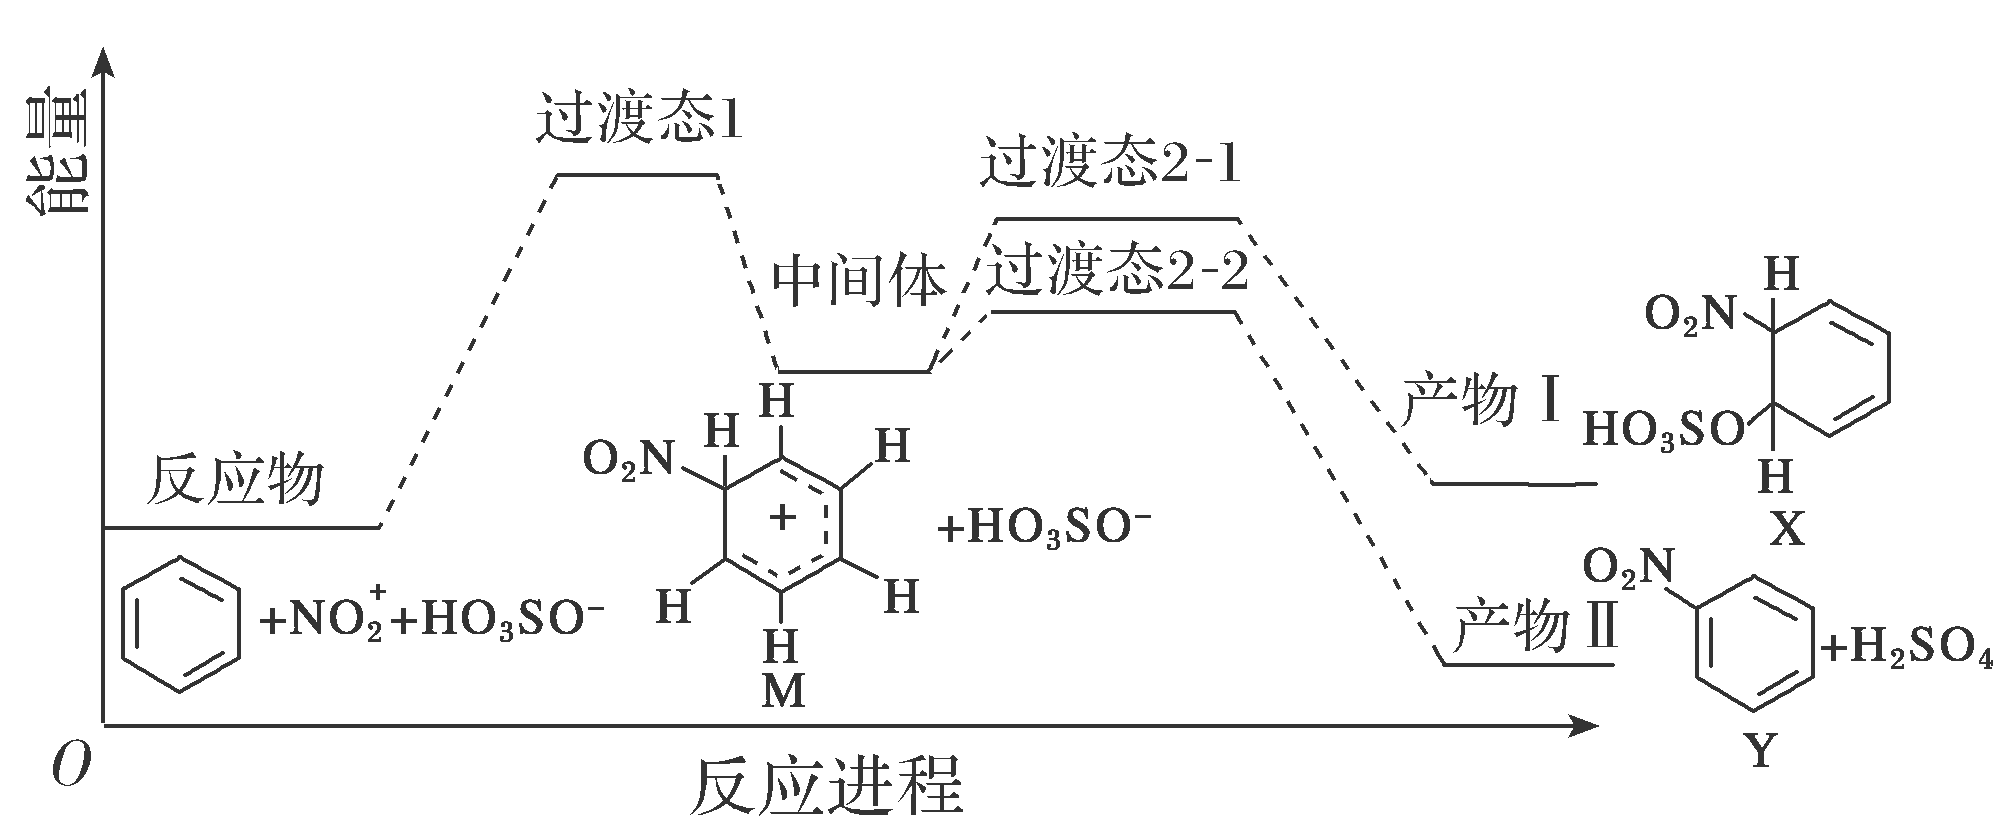
\includegraphics[width=0.5\textwidth]{assists/image12.png}
    \end{figure}
    \begin{adjustwidth}{4em}{}
        \begin{asparaenum}[A. ]
            \item 从中间体到产物,无论从产物稳定性还是反应速率的角度均有利于产物\Romannumeral{2}
            \item X为苯的加成产物,Y为苯的取代产物
            \item 由苯得到M时,苯中的大$\pi$键没有变化
            \item 对于生成Y的反应,浓$\ce{H2SO4}$作催化剂
        \end{asparaenum}
    \end{adjustwidth}
    \begin{answer}
        C
    \end{answer}
    \begin{point}
        化学反应中的能量变化、有机反应类型、催化剂
    \end{point}
    \begin{explanation}
        产物\Romannumeral{2}能量更低,更稳定,生成过渡态2-2能垒更低,反应速率更快,A选项正确;X为苯与硝酸、硫酸的加成产物,Y为苯与硝酸的取代产物,B选项正确;形成中间体时,其中一个碳原子由$sp^2$杂化转为$sp^3$杂化,苯的大$\pi$键由$\pi^6_6$转为$\pi^5_5$,C选项错误;硫酸在反应前后没有消耗,为催化剂,D选项正确。
    \end{explanation}
\end{subexercise}
\begin{subexercise}
    甲苯与氯气光照反应方程式为\blank 甲苯与液溴催化反应(一取代)方程式为\blank 甲苯与液溴催化反应(多取代)方程式为\blank 对比结论:\blank 结构角度解释:\blank 萘的结构式为\blank ,物理性质\blank 用途\blank 蒽的结构式为\blank ,物理性质\blank 用途\blank

    \begin{answer}
        \begin{inparaenum}[\quad\textsuperscript{\arabic{enumi}}]
            \item[\setcounter{enumi}{1}\textsuperscript{\arabic{enumi}}] $\chemfig{[,0.4]*6(-=-=(-)-=)} \ce{+ Cl2 ->T[光照] } \chemfig{[,0.4]*6(-=-=(--[:30]Cl)-=)} \ce{+ HCl}$\chdots\\
            \item $\chemfig{[,0.4]*6(-=-=(-)-=)}\ce{+ Br2 ->T[ \ce{FeBr3} ] HBr +} \chemfig{[,0.4]*6(-=-(-Br)=(-)-=)}$(主要)、$\chemfig{[,0.4]*6(-=-=(-)-=)}\ce{+ Br2 ->T[ \ce{FeBr3} ] HBr +} \chemfig{[,0.4]*6(-(-Br)=-=(-)-=)}$(次要)\\
            \item  $\chemfig{[,0.4]*6(-=-=(-)-=)}\ce{+ Br2 ->T[ \ce{FeBr3} ] HBr +} \chemfig{[,0.4]*6(-(-Br)=-(-Br)=(-)-(-Br)=)}$
            \item 产物可受反应条件调控
            \item $\ce{FeBr3}$可以极化甲苯,催化亲电加成反应;光照引发氯气均裂,生成氯自由基,催化自由基取代反应
            \item $\chemfig{[,0.4] *6(-=(*6(-=-=-))-=-=)}$
            \item 无色片状晶体,有特殊气味,熔点 80$^\circ$C,易升华,不溶于水
            \item 曾用于杀菌、防蛀、驱虫(有一定毒性,现已不再使用)
            \item $\chemfig{[,0.4] *6(-=(*6(-=-=-))-=-(*6(-=-=-))=)}$
            \item 无色晶体,易升华,不溶于水,易溶于苯
            \item 合成染料的重要原料
        \end{inparaenum}
    \end{answer}
\end{subexercise}
\setcounter{subexercise}{0}
\addtocounter{exercise}{1}
\begin{subexercise}
    \begin{multicols}{2}
        \noindent 完48页第1题(有机物物理性质)\\
        完成48页第2题(原子共面问题)\\
        完成48页第3题(有机化学反应类型判断)\\
        完成49页第4题(苯的同系物判断)\\
        完成49页5题(苯和甲苯鉴别)
    \end{multicols}
    \begin{answer}
        \fs{略}
    \end{answer}
\end{subexercise}
\begin{subexercise}
    \fs{[2024·安徽卷]}下列各组物质的鉴别方法中,不可行的是\quad (\quad)
    \begin{adjustwidth}{4em}{}
        \begin{asparaenum}[A. ]
            \item 过氧化钠和硫黄:加水,振荡
            \item 水晶和玻璃:X射线衍射实验
            \item 氯化钠和氯化钾:焰色试验
            \item 苯和甲苯:滴加溴水,振荡
        \end{asparaenum}
    \end{adjustwidth}
    \begin{answer}
        D
    \end{answer}
    \begin{point}
        物质鉴别(物理性质、化学性质)
    \end{point}
    \begin{explanation}
        过氧化钠与水反应生成氧气,可以观察到固体消失、产生气泡,硫磺入水没有明显实验现象,可以通过现象区分两者,A选项正确;水晶是晶体,玻璃是非晶体,在X射线衍射图谱中,通过晶体可以观察到明锐的谱线而非晶体不会的现象可以区分二者,B选项正确;钠的焰色为黄色,钾的焰色为紫色(透过蓝色钴玻璃),通过焰色不同可以区分,C选项正确;苯与甲苯滴加溴水振荡后现象均为溶液分层,上层为橙红色,下层颜色变浅或褪色,无法鉴别,D选项不符合题意。
    \end{explanation}
\end{subexercise}

\begin{exercise}
    \begin{multicols}{2}
        \noindent 完成49页第6题(含苯环的一氯代物种类)\\
        完成49页第7题(有机物命名)\\
        完成49页第8题(结构式与分子式)\\
        完成49页第9题(苯的同系物)\\
        完成49页第10题(芳香烃的取代反应)\\
        完成49页第11题(苯的同系物被高锰酸钾反应)\\
        完51页第1题(分离方式的选择)\\
        完成51页第2题(有机物性质与反应)\\
        完成51页第3题(有机分子中原子共面问题)\\
        完成51页第4题(核磁共振氢谱,不同环境的氢原子)\\
        完成51页5题(有机产物官能团)\\
        完成51页第6题(李比希元素分析)\\
        完成51页第7题(有机反应与化学键断裂)\\
        完成52页第8题(甲苯与酸性高锰酸钾反应的结构解释)\\
        完成52页第9题(一氯乙烷的制备与平均价)\\
        完成52页第10题(乙炔合成具丙烯腈)\\
        完成52页第11题(有机物反应推断)\\
    \end{multicols}
    \begin{answer}
        \fs{略}
    \end{answer}
\end{exercise}
\begin{exercise}
    \blank 叫做卤代烃。写出氯乙烯、二氯乙烷、2-氯乙烷、1,2-二溴乙烷的结构式\blank 。卤代烃,除\blank 外,大多数为液态和固态,一氯戊烷\blank 溶于水,可溶于有机溶剂,密度比水\blank ,溴乙烷密度比水\blank 。液化氯乙烷汽化时大量吸热,具有\blank 作用,复方氯乙烷气雾剂,用于运动中急性损伤。

    \begin{answer}
        \begin{inparaenum}[\quad\textsuperscript{\arabic{enumi}}]
            \item[\setcounter{enumi}{1}\textsuperscript{\arabic{enumi}}] 烃分子中的氢原子被卤素原子取代后生成的化合物
            \item $\chemfig{C(-[:120,0.5]Cl)(-[:240,0.5]H)=[,0.6]C(-[:60,0.5]H)(-[:300,0.5]H)}$;$\chemfig{[,0.6]C(-[2]Cl)(-[4]H)(-[6]H)-C(-H)(-[2]Cl)(-[6]H)}$或$\chemfig{[,0.6]C(-[2]Cl)(-[4]H)(-[6]Cl)-C(-H)(-[2]H)(-[6]H)}$;$\chemfig{[,0.6]C(-[2]H)(-[4]H)(-[6]H)-C(-H)(-[2]Cl)(-[6]H)}$;$\chemfig{[,0.6]C(-[2]Br)(-[4]H)(-[6]H)-C(-H)(-[2]Br)(-[6]H)}$
            \item 一氯甲烷
            \item 难
            \item 小
            \item 大
            \item 冷冻麻醉
        \end{inparaenum}
    \end{answer}
    \begin{note}
        题\textsuperscript{2}中“2-氯乙烷”是不符合IPUAC命名规则的,这里按照“氯乙烷”给出答案。
    \end{note}
\end{exercise}
\begin{exercise}
    阅读并完成55页实验3-1中的内容,实验现象为\blank ,水解反应为\blank ,加硝酸的目的是\blank 。从极性键角度解释水解反应机理:\blank 溴乙烷与强碱的乙醇溶液反应的化学方程式为\blank 。\blank 叫做消去反应。阅读并完成56页探究实验的表格,1-溴丁烷生成丁醇的反应为\blank ,哪种分析手段可检测生成了丁醇\blank ,1-溴丁烷生成丁烯的反应类型为\blank ,反应方程式为\blank ,检验产物:\blank 。讨论1:\blank ,讨论2:\blank 。聚氯乙烯和聚四氟乙烯生成的方程式\blank 反应类型为\blank ,用途为(各举一例)\blank 。氟利昂对臭氧层破坏的机理:\blank
    \begin{answer}
        \begin{inparaenum}[\quad\textsuperscript{\arabic{enumi}}]
            \item[\setcounter{enumi}{1}\textsuperscript{\arabic{enumi}}] 有浅黄色沉淀
            \item $\ce{R-X + OH- ->T[水][$\triangle$] R-OH + Br-}$
            \item 中和碱,排除对卤素检验的干扰
            \item 由于电负性差异,R基团略微带正电,$\ce{OH-}$进攻R基团发生亲核取代,随后卤素原子脱落为离子
            \item $\ce{CH3CH2-Br + MOH ->T[乙醇][$\triangle$] MBr + H2O + CH2=CH2}$
            \item 有机物在一定条件下,从一个分子中脱去一个或几个小分子,而生成含不饱和键的反应
            \item $\chemfig{[,0.5] -[:30](-[2]Br)-[:-30]-[:30]}\ce{+ NaOH ->T[水][$\triangle$] NaBr + }\chemfig{[,0.5] -[:30](-[2]OH)-[:-30]-[:30]}$
            \item 化学分析法(\textbf{Lucas试剂}等)、红外光谱仪、核磁共振氢谱\chdots
            \item 消去反应
            \item $\chemfig{[,0.5] -[:30](-[2]Br)-[:-30]-[:30]}\ce{NaOH + ->T[乙醇][$\triangle$] H2O + NaBr + }\chemfig{[,0.5] =-[:30]-[:-30]}$
            \item 将丁烯通入溴的四氯化碳溶液中,观察到溶液褪色
            \item 乙醇有还原性,排除对产物检验的干扰
            \item 1-丁烯、2-丁烯
            \item $\ce{n CH2=CHCl ->T[CAT] }\chemfig{[,0.6]-[@{left,0.5}]CH_2-CHCl-[@{right,0.5}]}\polymerdelim[delimiters={[]},height=5pt, depth=5pt, indice=n]{left}{right}$、$\ce{n CF2=CF2 ->T[CAT] }\chemfig{[,0.6]-[@{left,0.5}]CF_2-CF_2-[@{right,0.5}]}\polymerdelim[delimiters={[]},height=5pt, depth=5pt, indice=n]{left}{right}$
            \item 加成聚合反应\vspace{0.5em}
            \item 管材、薄膜;不粘锅、防水外衣等
            \item $\ce{O3 <=>T[紫外线] O2 + }\charge{0=\.}{\ce{O}}\hspace{0.5em}$、$\ce{CCl3F ->T[紫外线] }\charge{0=\.}{\ce{CCl2F}}\hspace{0.5em}\charge{0=\.}{\ce{+ Cl}}\hspace{0.5em}$、$\charge{0=\.}{\ce{Cl}}\hspace{0.5em}\ce{+ O3 -> O2 + }\charge{0=\.}{\ce{ClO}}\hspace{0.5em}$、$\charge{0=\.}{\ce{ClO}}\hspace{0.5em}\ce{+}\charge{0=\.}{\ce{O}}\hspace{0.5em}\ce{-> O2 + }\charge{0=\.}{\ce{Cl}}\hspace{0.5em}$
        \end{inparaenum}
    \end{answer}
    \begin{note}
        \textbf{Lucas试剂:}由浓盐酸和无水氯化锌组成,可以鉴别叔醇、仲醇,反应形成不溶于酸的卤代烃油状物,溶液变混浊并分层。题\textsuperscript{13}未考虑立体异构。
    \end{note}
\end{exercise}
\begin{exercise}
    \begin{multicols}{2}
        \noindent 完58页第1题(卤代烃的性质)\\
        完成58页第2题(同系物判断)\\
        完成58页第3题(卤代烃的消去反应)\\
        完成58页第4题(取代反应判断)\\
        完成58页5题(检验卤代烃中卤素的实验操作)\\
        完成58页第6题(卤代烃消去和取代反应方程式书写)\\
        完成58页第7题(通过计算进行有机物推断)\\
        完成58页第8题(有机物推断)\\
        完成58页第9题(有机合成路线)
    \end{multicols}
    \begin{answer}
        \fs{略}
    \end{answer}
\end{exercise}
\setcounter{subexercise}{0}
\addtocounter{exercise}{1}
\begin{subexercise}
    写出正丙醇、2-丙醇、乙二醇、丙三醇、1,3-丙二醇、苯甲醇、邻甲基苯酚、3-甲基-2-乙基苯酚的结构式\blank 甲醇与水互溶是因为\blank 甲醇有毒是因为\blank 乙二醇、甘油均是与水互溶且粘稠的液体是因为\blank 甲醇、乙烷的相对分子质量差不多,甲醇的沸点高的多的原因是\blank 从化学键断裂角度分析乙醇和浓氢溴酸的反应:\blank 阅读并完成61页3-2实验,乙醇的消去反应化学方程式为\blank ,为什么乙醇和浓硫酸体积1:3,\blank 加碎瓷片的作用\blank ,忘了加则应该\blank 为什么要迅速升温到170$^\circ$C\blank 可能的副反应为\blank 还有:\blank 如何控制温度\blank ,还可以如何做\blank 先通过氢氧化钠溶液再通过酸性高锰酸钾的目的是\blank 酸性高锰酸钾和溴的四氯化碳的作用和现象分别是\blank 溴乙烷和乙醇的消去反应有什么异同\blank 乙醚和乙醇互为\blank ,但乙醚更易挥发是因为\blank 乙醇和乙醚均能与水互溶是因为\blank 乙醚常做麻醉剂,是一种良好的有机溶剂,但闪点极低,易燃易爆,实验时应注意\blank 甲醚的结构式为\blank ,苯甲醚的结构式为\blank ,甲乙醚的结构式为\blank 写出$\ce{C3H8O}$的同分异构体结构简式和名称\blank
    \begin{answer}
        \begin{inparaenum}[\quad\textsuperscript{\arabic{enumi}}]
            \item[\setcounter{enumi}{1}\textsuperscript{\arabic{enumi}}]
            \chemfig{[,0.5] -[:30]-[:-30]-[:30]-[:-30]-OH}、
            \chemfig{[,0.5] -[:30](-[2])-[:-30]-OH}、
            \chemfig{[,0.6] CH_2(-[2]OH)-CH_2(-[2]OH)}、
            \chemfig{[,0.5] HO--[:30](-[2]OH)-[:-30]-OH}、
            \chemfig{[,0.5] HO--[:30]-[:-30]-OH}、
            \chemfig{[,0.4] *6(-=-=(--[:30]OH)-=)}、
            \chemfig{[,0.4] *6(-=-(-OH)=(-)-=)}、
            \chemfig{[,0.4] *6(-=(-)-(--[:0])=(-OH)-=)}
            \item 甲醇含有羟基,分子极性大,相似相溶于极性溶剂水
            \item 在体内代谢为甲醛,进而转化为甲酸累积于血液中,引发代谢性酸中毒;抑制线粒体内细胞色素氧化酶活性,阻碍有氧呼吸。
            \item 均含有羟基,分子极性大,相似相溶于极性溶剂水;且可以形成分子间氢键,故粘稠
            \item 能够形成分子间氢键,沸点更高
            \item 浓氢溴酸电离提供质子使乙醇质子化($\ce{C2H5OH2^+}$),再脱去一分子水形成中间体$\ce{C2H5^+}$,最后与溴离子结合
            \item $\ce{CH3CH2OH ->T[浓硫酸][$\triangle$] CH2=CH2 ^ + H2O}$
            \item 充分的催化、脱水能力,抑制副反应
            \item 防止暴沸
            \item 将体系冷却后补加
            \item 避免发生副反应
            \item $\ce{2 CH3CH2OH ->T[浓硫酸][140$^\circ$C] H2O + CH3CH2OCH2CH3}$
            \item $\ce{C2H5OH + 2 H2SO4 -> 2C v + 2SO2 ^  + CO2 ^ + 4H2O}$、$\ce{CH3CH2OH + H2SO4 -> CH3CH2OSO3H + H2O}$
            \item 油浴加热
            \item 水蒸气加热
            \item 避免乙醇影响乙烯的检验
            \item 检验还原性,褪色;验证加成反应,褪色
            \item 异:双分子消去反应(E2消去):碱的醇溶液、副反应亲核取代 vs 单分子消去反应(E1消去):浓硫酸较高温度、副反应分子间脱水 $||$ 同:\fs{略}
            \item 同分异构体
            \item 乙醇容易形成氢键,且分子极性较大有微弱电性作用,故更不易挥发
            \item 乙醇含有羟基,分子极性大,相似相溶于极性溶剂水,另外可与水形成氢键;乙醚有氧原子,可以作为氢键受体,溶于水
            \item 使用乙醚时应严格防静电、远离明火,保存乙\vspace{0.5em}醚时应密封、避光、低温、远离氧化剂与火源
            \item $\ce{CH3OCH3}$
            \item $\chemfig{[,0.4] *6(-=-(-OCH_3)=-=)}$
            \item $\ce{CH3CH2OCH3}$
            \item
            $\mathop{\ce{CH3CH2CH2OH}}\limits_{\mbox{\kaishu 正丙醇}}$、
            $\mathop{\ce{CH3CH(OH)CH3}}\limits_{\mbox{\kaishu 异丙醇}}$、
            $\mathop{\ce{CH3CH2OCH3}}\limits_{\mbox{\kaishu 甲乙醚}}$
        \end{inparaenum}
    \end{answer}
\end{subexercise}
\begin{subexercise}
    \fs{[2022·6月浙江选考]}下列反应的离子方程式不正确的是\quad (\quad)
    \begin{adjustwidth}{4em}{}
        \begin{asparaenum}[A. ]
            \item 盐酸中滴加$\ce{Na2SiO3}$溶液:$\ce{SiO3^2- + 2H+ = H2SiO3 v}$
            \item $\ce{Na2CO3}$溶液中通入过量$\ce{SO2}$:$\ce{CO3^2- + 2SO2 + H2O = 2HSO3^- + CO2}$
            \item 乙醇与$\ce{K2Cr2O7}$酸性溶液反应:$\ce{3CH3CH2OH + 2Cr2O7^2- + 16H+ -> 3CH3COOH + 4Cr^3+ + 11H2O}$
            \item 溴与冷的$\ce{NaOH}$溶液反应:\ce{Br2 + OH- = Br- + BrO- + H+}
        \end{asparaenum}
    \end{adjustwidth}
    \begin{answer}
        D
    \end{answer}
    \begin{point}
        离子方程式的书写
    \end{point}
    \begin{explanation}
        在碱性环境中氢离子不能作生成物,D选项错误。
    \end{explanation}
\end{subexercise}
\begin{subexercise}
    乙醇在人体内的氧化为:\blank 苯酚是无色晶体但放置在空气中时间过长容易出现粉红色是因为\blank 室温下苯酚溶解度9.2g,65$^\circ$C以上与水互溶是因为\blank 苯酚沾到皮肤上立即乙醇冲洗再水洗是因为\blank 阅读并完成64页实验3-4中的表格,化学方程式为\blank 、\blank 实验现象为:\blank 、\blank 从结构上解释苯酚显弱酸性俗称石碳酸是因为\blank 苯酚钠中通入二氧化碳现象为\blank ,离子方程式为\blank 继续通入过量的二氧化碳现象为\blank ,原因是\blank 说明了\blank 阅读并完成65页实验3-5,实验现象为\blank ,化学方程式为\blank 滴加饱和溴水的目的是\blank 从结构上解释该反应进行的原因是:\blank 苯酚与溴的反应和灵敏,可用于\blank 从分子内基团相互影响解释:乙酸酸性强于碳酸强于苯酚强于乙醇\blank 苯和苯酚发生溴代反应的条件和产物有很大的不同\blank
    \begin{answer}
        \begin{inparaenum}[\quad\textsuperscript{\arabic{enumi}}]
            \item[\setcounter{enumi}{1}\textsuperscript{\arabic{enumi}}] 乙醇$\ce{->T[乙醇脱氢酶]}$乙醛$\ce{->T[乙醛脱氢酶]}$乙酸
            \item 被空气中氧气氧化形成醌类物质\vspace{0.5em}
            \item 可与水形成氢键
            \item 苯酚在乙醇中溶解度更大,洗去苯酚效果更好
            \item $\chemfig{[,0.4] *6(-=-=(-OH)-=)}\ce{ + NaOH -> H2O + }\chemfig{[,0.4] *6(-=-=(-ONa)-=)}$
            \item $\chemfig{[,0.4] *6(-=-=(-ONa)-=)}\ce{+ HCl -> NaCl + }\chemfig{[,0.4] *6(-=-=(-OH)-=)}$
            \item 白色沉淀溶解
            \item 产生白色沉淀
            \item 氧原子电负性大,极化$\chemfig{O-H}$键使氢原子易于电离;解离生成的苯氧负离子($\ce{C6H5O-}$)p-$\pi$共轭很稳定,故解离倾向性大
            \item 产生白色沉淀
            \item $\ce{H2O + CO2 + PhO- -> HCO3^- + PhOH v }$
            \item 析出白色晶体
            \item $\ce{NaHCO3}$在水中溶解度小
            \item 苯酚的酸性界于碳酸和碳酸氢根之间
            \item 产生白色絮状沉淀
            \item $\chemfig{[,0.4] *6(-=-=(-OH)-=)}\ce{+ 3Br2 -> }\chemfig{[,0.4] *6(-(-Br)=-(-Br)=(-OH)-(-Br)=)}\ce{v + 3HBr}$
            \item 抑制副产物,使反应现象显著
            \item 羟基是邻对位定位基,活化邻对位
            \item 检验苯酚
            \item 乙酸:有亚氧基($\ce{=O}$)拉电子基团;碳酸:有亚氧基拉电子,但对称性较高,溶解度也较低;苯酚:氧原子电负性大,极化$\ce{O-H}$键使氢原子易于电离,且解离生成的苯氧负离子($\ce{C6H5O-}$)p-$\pi$共轭很稳定,故解离倾向性大;乙醇:甲基为推电子基团,减小了$\ce{O-H}$的极性
            \item 羟基是邻对位定位基,活化邻对位
        \end{inparaenum}
    \end{answer}
\end{subexercise}
\begin{subexercise}
    \fs{[2024甘肃卷]}温室气体$\ce{N2O}$在催化剂作用下可分解为$\ce{O2}$和$\ce{N2}$,也可作为氧化剂氧化苯制苯酚,下列说法错误的是\quad(\quad)
    \begin{adjustwidth}{4em}{}
            \begin{asparaenum}[A. ]
                \item 原子半径:O<N<C
                \item 第一电离能:C<N<O 
                \item 在水中的溶解度:苯<苯酚
                \item 苯和苯酚中C的杂化方式相同
            \end{asparaenum}
    \end{adjustwidth}
    \begin{answer}
        B
    \end{answer}
    \begin{point}
        原子半径、第一电离能、氢键、杂化方式
    \end{point}
    \begin{explanation}
        N的p轨道半满,比O的电离能大,原子半径:C<O<N,故B选项错误。
    \end{explanation}
\end{subexercise}
\begin{subexercise}
        阅读并完成62页实验3-5,实验现象为\blank ,化学方程式为\blank 是否所有酚类物质均可用氯化铁检验\blank 为什么酸性过强的溶液要先中和,再加氯化铁溶液检验\blank 苯酚可以用于制造酚醛树脂,反应方程式为\blank 苯酚可用于外用消毒是因为\blank 。化工厂和炼焦厂的废水中常含有酚类物质,在排放前须\blank ,可以选用\blank 作试剂。
        \begin{answer}
            \begin{inparaenum}[\quad\textsuperscript{\arabic{enumi}}]
                \item[\setcounter{enumi}{1}\textsuperscript{\arabic{enumi}}] 由橙红色变为灰绿色
                \item $\ce{3CH3CH2OH + K2Cr2O7 + 4H2SO4 -> 3CH3CHO + K2SO4 + Cr2(SO4)3 + 7H2O}$、$\ce{3CH3CH2OH + 2K2Cr2O7 + 8H2SO4 -> 3CH3COOH + 2K2SO4 + 2Cr2(SO4)3 + 11H2O}$
                \item 不是,要与$\ce{Fe^3+}$发生显色反应,分子中必须存在能与$\ce{Fe^3+}$发生作用的电子体系,通常是具有共轭结构的烯醇式结构,如2,4,6-三叔丁基苯酚就因空间位阻无法形成有效的配位,因此通常不显色。
                \item 因为酚类发生配位的有效物质主要是$\ce{PhO-}$,而不是$\ce{PhOH}$,若酸性过强,前者在溶液中的浓度较低,不易发生明显的配位(显色)反应。\vspace{0.5em}\\
                \item $\chemfig{[,0.5] *6(-=-=(-OH)-=)} \ce{+ HCHO ->T[$\ce{H+}$][$\triangle$] }\chemfig{[,0.4]*6(-=-(-CH_2OH)=(-OH)-=)}$、$\chemfig{[,0.4]*6(-=-(-CH_2OH)=(-OH)-=)}\ce{->T[$\ce{H+}$][$\triangle$] (n-1) H2O +}\chemfig{[,0.4] *6(-=-(-CH_2-[@{right,0.5}:0,0.8]OH)=(-OH)-(-[@{left,0.5}:180,0.8]H)=) }\polymerdelim[delimiters={[]},height=15pt, depth=15pt, h align=false, indice=n]{left}{right}$ \\
                \item 使微生物的蛋白质变性或凝固、破坏细胞膜/细胞壁、抑制特定酶系统
                \item 进行处理以降解或去除酚
                \item 氧化剂(如臭氧、氯气、过氧化氢等)或特种微生物(活性污泥法)
            \end{inparaenum}
        \end{answer}
\end{subexercise}
\begin{exercise}
        \begin{multicols}{2}
\noindent 完67页第1题(醇和酚区别)\\
完成67页第2题(苯酚显酸性的原因)\\
完成67页第3题(分子内基团相互影响)\\
完成67页第4题(醇的性质)\\
完成67页5题(分子间氢键对醇的熔沸点和溶解度影响)\\
完成67页第6题(常见有机物相互转化关系)\\
完成67页第7题(苯酚和铁离子配位作用)\\
完成67页第8题(设计对种方案鉴别苯和苯酚)\\
完成67页第9题(通过计算进行有机物推断)\\
完成67页第10题(六元环状有机物合成路线)
    \end{multicols}
    \begin{answer}
        \fs{略}
    \end{answer}
\end{exercise}

\end{document}
